\documentclass{article}

\usepackage[utf8]{inputenc}
\usepackage[margin=1.25in]{geometry}
\usepackage{amsmath, amssymb, amsthm}
\usepackage{graphicx}
\usepackage{mathdots}
\usepackage{esvect}
\setlength{\parskip}{1em}
\setlength{\parindent}{2em}
\usepackage{indentfirst}
\usepackage{matlab-prettifier}
\usepackage[T1]{fontenc}

\begin{document}

\begin{titlepage}
\centering
	\vspace*{\fill}
	{\huge\bfseries ROB521 A3 - Lidar Mapping \& Localization\par}
	\vspace{7cm}
	{\Large\itshape Ethan Rajah\par}
	{\Large April 7, 2025\par}
	\vspace*{\fill}
\end{titlepage}

\newpage
\section{Question 1}
This question required the implementation of an occupancy grid mapping algorithm using Lidar data to build a map of the environment.
This required tracing lidar distance measurements from the current robot pose at each timestep during the robots motion and updating a probability grid map based on the
if cells were occupied or not. More specifically, the algorithm marks free space grid indices along the ray traced by the Lidar sensor from the current robot pose by decrementing
the probability of occupancy of the cell by 0.5, and marks occupied space grid indices (the end points of the ray denoted by the Lidar scan) by incrementing the probability of occupancy of the cell by 1.5.
These values were tuned by running the algorithm and observing how defined the free (white) and occupied (black) space was in the resulting map.
Finally, the logits are converted into probabilities using the sigmoid function. The resulting map is shown in \textbf{Figure 1}.
The figure shows that this algorithm is able to build a map of complex environments with high accuracy, maintaining the structure of the robot's surroundings.

\begin{figure}[h!]
    \centering
    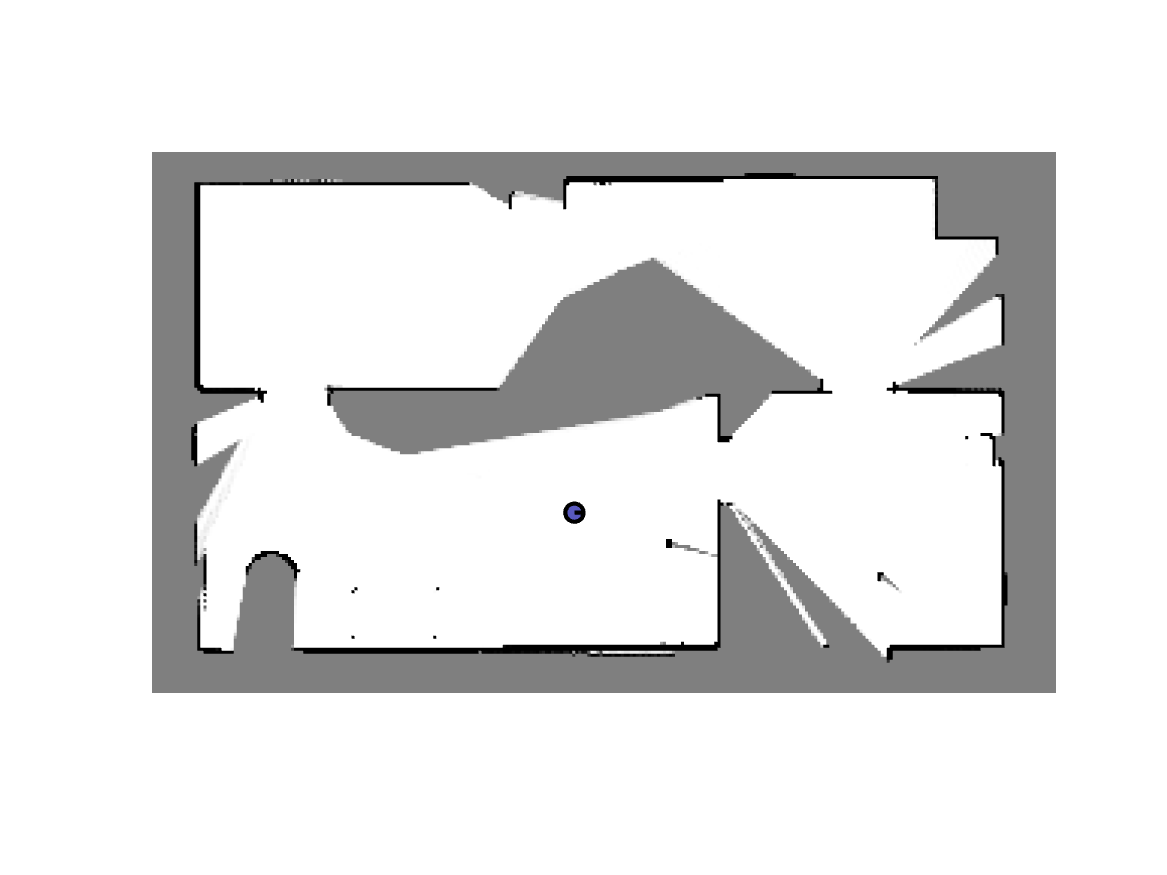
\includegraphics[width=0.8\textwidth]{ass2_q1.png}
    \caption{Built map from occupancy grid mapping algorithm and Lidar data.}
\end{figure}

\section{Question 2}
This question required the implementation of a particle filter algorithm to localize a robot in a known map using Lidar data.
The algorithm initializes a set of particles in the map, and at each timestep, the particles are propagated through a motion model using the odometry data and corrected using the Lidar data.
The particles are weighted based on how likely they are to be in the correct position given the current Lidar measurements. This is done by
reweighing the particles at each timestep based on their residual error from the propagated predicted measurement given the predicted pose
and the actual Lidar measurement. Similar to Question 1, the measurements at each timestep are ray traced based on the estimated pose of the particle
to obtain the closest occupied cell in the map. The actual measurement is set as the mean of a Gaussian distribution defining the likelihood of the particle given the measurement,
and the predicted measurement is used to aid in forming the PDF, which is then used to reweigh the particles. The particles are then resampled based on their weights to ensure that the particles
with higher weights are more likely to be selected. The resulting map is shown in \textbf{Figure 2}, which shows the localization error between the odometry estimates and the particle filter estimates.
The figure shows that the particle filtering technique is far superior to odometry estimates, as the localization error is significantly lower on average.

\begin{figure}[h!]
    \centering
    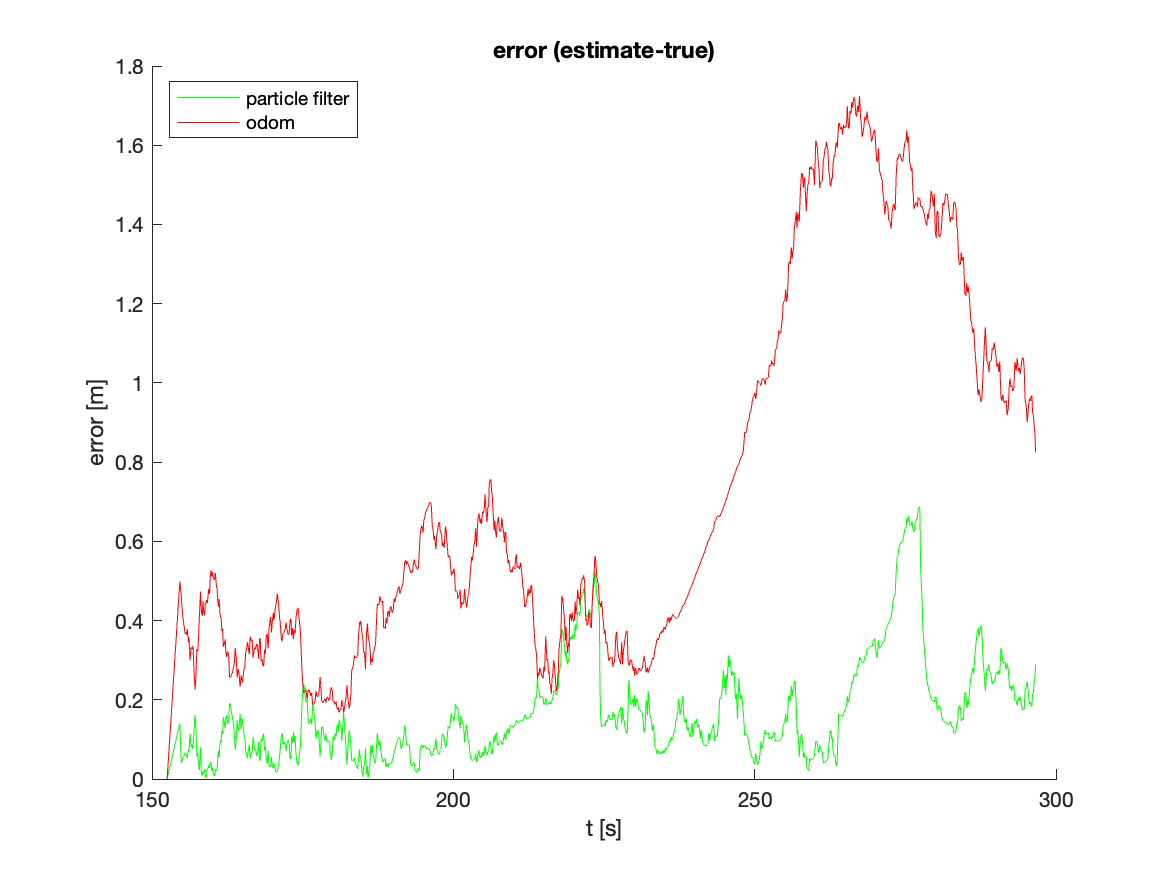
\includegraphics[width=0.8\textwidth]{ass2_q2.png}
    \caption{Localization error comparison between odometry estimates and particle filter estimates.}
\end{figure}

\section{MATLAB Code}

The MATLAB code for these implementations are provided here, as well as are attached in the submission.

\lstinputlisting[
frame=single,
numbers=left,
style=Matlab-editor
]{ass3_q1.m}

\lstinputlisting[
frame=single,
numbers=left,
style=Matlab-editor
]{ass3_q2.m}

\end{document}